%%% Sekce – Interaktivní mapa sedadel
%%%%% Wording: ⏳
%%%%% Styling: ⏳
%%%%% References: ⏳
%%% --------------------------------------------------------------
\section{Interaktivní mapa sedadel}
\label{sec:implementace-seating}
Vývoj webové aplikace zahrnuje několik klíčových prvků, z nichž každý představuje jedinečné výzvy a příležitosti k učení.
Tyto prvky jsou základem funkčnosti aplikace a každý z nich hraje klíčovou roli při zlepšování uživatelské zkušenosti.
Vývoj těchto prvků vyžadoval pevné porozumění frontendovým technologiím, jejich možnostem, omezením a osvědčeným postupům.

Jedním z těchto klíčových prvků je interaktivní mapa sedadel.
Tato funkce umožňuje uživateli vizuálně procházet uspořádáním sedadel v místnosti a vybrat si své preferované místo.
Mapa sedadel uživatelům poskytuje přehled o všech dostupných sedadlech, jejich kategoriích a stavech, čímž usnadňuje proces rozhodování.
Tato funkce výrazně zlepšuje uživatelskou zkušenost tím, že poskytuje intuitivní a interaktivní rozhraní pro výběr sedadel.

%%% Podsekce – Struktura
%%%%% Wording: ⏳
%%%%% Styling: ⏳
%%%%% References: ⏳
%%% --------------------------------------------------------------
\subsection{Struktura}
\label{subsec:implementace-seating-struktura}
Struktura této funkce je postavena na několika komponentech, které spolu harmonicky spolupracují.
Primárními komponentami jsou:

\begin{itemize}
	\item SeatingMapProvider
	\item SeatingMap
	\item VirtualMap
	\item Seat
	\item SeatSheet
\end{itemize}

\textbf{SeatingMapProvider} je nadřazená komponenta, která získává data z API a zpřístupňuje je ostatním komponentám.
Tato data zahrnují podrobnosti o místnosti, sedadlech, jejich stavech a přidružených vstupenkách.

\textbf{SeatingMap} je komponenta, která zpracovává SVG data.
Přebírá SVG data z API a překládá je do formátu, který může být použit komponentou VirtualMap.

\textbf{VirtualMap} je zodpovědná za přidání interaktivity do SeatingMap.
Umožňuje funkce, jako je posouvání, přibližování a oddalování mapy, čímž poskytuje dynamický uživatelský zážitek.

\textbf{Seat} a \textbf{SeatSheet} komponenty představují jednotlivá sedadla na mapě a podrobnosti zobrazené při výběru sedadla.

\begin{minted}[breaklines]{jsx}
<SeatingMapProvider venue={venue}>
	{/* seating map */}
	<SeatingMap width={width} height={height}>
		{/* virtual map */}
		<VirtualMap minScaleFactor={1.1} maxScaleFactor={0.1}>
			{/* individual seats */}
			<Seat />
			<Seat />
			<Seat />
			{/* + any other svg elements */}
		</VirtualMap>

		{/* seat sheet detail */}
		<Sheet>
			<Sheet.Header />
			<Sheet.Body>
				<SeatSheetDetail />
			</Sheet.Body>
		</Sheet>
	</SeatingMap>
</SeatingMapProvider>
\end{minted}

%%% Podsekce – Získávání a správa dat
%%%%% Wording: ⏳
%%%%% Styling: ⏳
%%%%% References: ⏳
%%% --------------------------------------------------------------
\subsection{Získávání a správa dat}
\label{subsec:implementace-seating-data}
Proces získávání a správy dat začíná komponentou SeatingMapProvider.
Tato komponenta vytvoří požadavek na API, aby získala data týkající se uspořádání sedadel v místnosti.

\begin{minted}[breaklines]{typescript}
/**
 * Venue API response schema
 * @export
 */
export const venueApiSchema = z.object({
	/** venue id */
	venueId: z.string().uuid(),
	/** venue name */
	name: z.string(),
	/** seating drawing (SVG) */
	drawing: z.string(),
	/** venue seat data */
	seats: z.array(
		z.object({
			/** seat id */
			seatId: z.string().uuid(),
			/** seat row display label */
			row: z.string(),
			/** seat place number */
			place: z.number(),
			/** seat full display name label */
			fullName: z.string(),
			/** seat available capacity left */
			capacityLeft: z.number(),
			tickets: z.array(z.string().uuid()),
			categoryId: z.string().uuid(),
		}),
	),
	/** venue ticket data */
	tickets: z.array(
		z.object({
			/** ticket id */
			ticketId: z.string().uuid(),
			name: z.string(),
			description: z.string().optional(),
			price: z.number().int(),
			categories: z.array(
				z.object({
					categoryId: z.string().uuid(),
					price: z.number().int(),
				}),
			),
		}),
	),
	/** venue ticket categories */
	categories: z.array(
		z.object({
			/** category id */
			categoryId: z.string().uuid(),
			name: z.string(),
			description: z.string().optional(),
			color: z.string(),
		}),
	),
});
\end{minted}

Odpověď API zahrnuje podrobnou SVG reprezentaci uspořádání sedadel v místnosti, jednotlivá data sedadel a přidružené vstupenky.
Každé sedadlo obsahuje informace o jeho řádku, místě, plném názvu, dostupné kapacitě a přidružených vstupenkách a kategoriích.
Každá vstupenka obsahuje informace o jejím id, názvu, volitelném popisu, ceně a kategoriích.

Po získání dat komponenta SeatingMapProvider zpracuje data do použitelnějšího formátu.
Toto zpracování zahrnuje oddělení sedadel, vstupenek a kategorií do vlastních struktur, vytvářející hierarchii, která zjednodušuje přístup k datům pro následující komponenty.

Tento zpracovaný formát je pak ostatním komponentám zpřístupněn pomocí kontextu, což poskytuje pohodlný způsob, jak k nim přistupovat.

%%% Podsekce – Parsování SVG a mapování sedadel
%%%%% Wording: ⏳
%%%%% Styling: ⏳
%%%%% References: ⏳
%%% --------------------------------------------------------------
\subsection{Parsování SVG a mapování sedadel}
\label{subsec:implementace-seating-svg}
SeatingMap komponenta je zodpovědná za parsování SVG dat a jejich překlad do formátu, který může být použit komponentou VirtualMap.

Tato komponenta přijímá SVG data z API a zpracovává je pomocí knihovny xml-js.
SVG data z API následují specifickou strukturu, kde `<g>` elementy představují skupiny sedadel, a tyto jsou identifikovány pomocí id atributu `seats:xxx`.
Jednotlivá sedadla v rámci těchto skupin jsou reprezentována `<circle>` elementy, identifikovanými jejich jedinečnými id ve formě `seat:row+place`.

% FIXME: svg comments broken
\begin{minted}{xml}
<svg width="1287" height="1115" viewBox="0 0 1287 1115" fill="#F2F4F7" xmlns="http://www.w3.org/2000/svg">
    <!-- seats -->
    <g id="seats:back">
        <!-- seat H+1 -->
        <circle id="seat:H+1" cx="48" cy="785" r="50" fill="#D0D5DD"/>
        <!-- seat I+1 -->
        <circle id="seat:I+1" cx="48" cy="805" r="50" fill="#D0D5DD"/>
        <!-- ...
-->
    </g>
    <g id="seats:right">
        <!-- ...
-->
    </g>
    <g id="seats:left">
        <!-- ...
-->
    </g>
    <g id="seats:center">
        <!-- ...
-->
    </g>
    <!-- details -->
    <g id="details:patio">
        <!-- ...
-->
    </g>
    <!-- ...
-->
</svg>
\end{minted}

Jakmile jsou SVG data zparsována, komponenta SeatingMap mapuje data sedadel na parsované SVG elementy, nahrazující každý `<circle>` element odpovídající komponentou <Seat>.
Každá komponenta <Seat> reprezentuje jedno sedadlo a zahrnuje všechna příslušná data pro toto sedadlo.

%%% Podsekce – Interaktivita s VirtualMap
%%%%% Wording: ⏳
%%%%% Styling: ⏳
%%%%% References: ⏳
%%% --------------------------------------------------------------
\subsection{Interaktivita s VirtualMap}
\label{subsec:implementace-seating-virtualmap}
Komponenta VirtualMap přidává interaktivitu do mapy sedadel.
Tato komponenta obaluje komponentu SeatingMap, přebírající parsované a namapované SVG elementy jako své potomky, a zajišťuje všechny interakce s mapou sedadel.


Tato komponenta využívá knihovny react-spring a use-gesture k implementaci interakcí s mapou sedadel.
Tyto knihovny umožňují plynulé a responzivní animace pro gesta panningu, zoomování a pinching, poskytující dynamický a plynulý uživatelský zážitek.

Komponenta VirtualMap také zajišťuje správu stavu mapy sedadel, sledováním změn, jako je úroveň zoomu, posunutí pan, a aktuálně vybrané sedadlo.
Tato správa stavu zajišťuje konzistentní uživatelský zážitek, i když je mapa sedadel manipulována uživatelem.

%%% Podsekce – Výběr sedadla a správa vstupenek
%%%%% Wording: ⏳
%%%%% Styling: ⏳
%%%%% References: ⏳
%%% --------------------------------------------------------------
\subsection{Výběr sedadla a správa vstupenek}
\label{subsec:implementace-seating-seat}
Komponenta Seat a SeatSheet jsou zodpovědné za výběr sedadla a správu vstupenek.

Komponenta Seat reprezentuje jednotlivá sedadla na mapě.
Každá komponenta Seat zahrnuje všechna příslušná data sedadla, jako je jeho dostupnost a aktuální stav.
Kliknutím na dostupné sedadlo můžou uživatelé zobrazit jeho detaily, včetně příslušných vstupenek.
Tato interakce spouští otevření komponenty SeatSheet, která poskytuje uživatelsky přívětivé rozhraní pro výběr vstupenky.

% TODO: screenshot of the Seat component
\begin{verbatim}
// TODO: screenshot of the SeatSheet component
\end{verbatim}

Komponenta SeatSheet zobrazuje detaily vybraného sedadla, včetně jeho kategorie, řádku, místa a dostupných vstupenek.
Vstupenky jsou vázány na kategorii sedadla a kategorie může mít několik příslušných vstupenek.
Cena vstupenky je definována kombinací její kategorie a vybraného sedadla.

Uživatel může přidat vybranou vstupenku do svého košíku přímo z rozhraní SeatSheet.
Pokud je v košíku již vstupenka pro vybrané sedadlo, může uživatel vybrat, zda chce vstupenku vyměnit nebo ji z košíku odebrat.
Všechny tyto změny se okamžitě promítají do komponenty SeatSheet, poskytující uživateli zpětnou vazbu v reálném čase.

Ve shrnutí je komponenta Interactive Seating Map kombinací načítání a správy dat, parsování SVG a mapování sedadel, interaktivity s VirtualMap a výběru sedadla a správy vstupenek.
Tyto komponenty spolupracují na vytvoření dynamické, interaktivní a uživatelsky přívětivé volby sedadel.
Výsledkem je vysoce flexibilní a intuitivní systém, který zjednodušuje proces výběru vstupenek a správu košíku.

\begin{figure}[h]
	\centering
	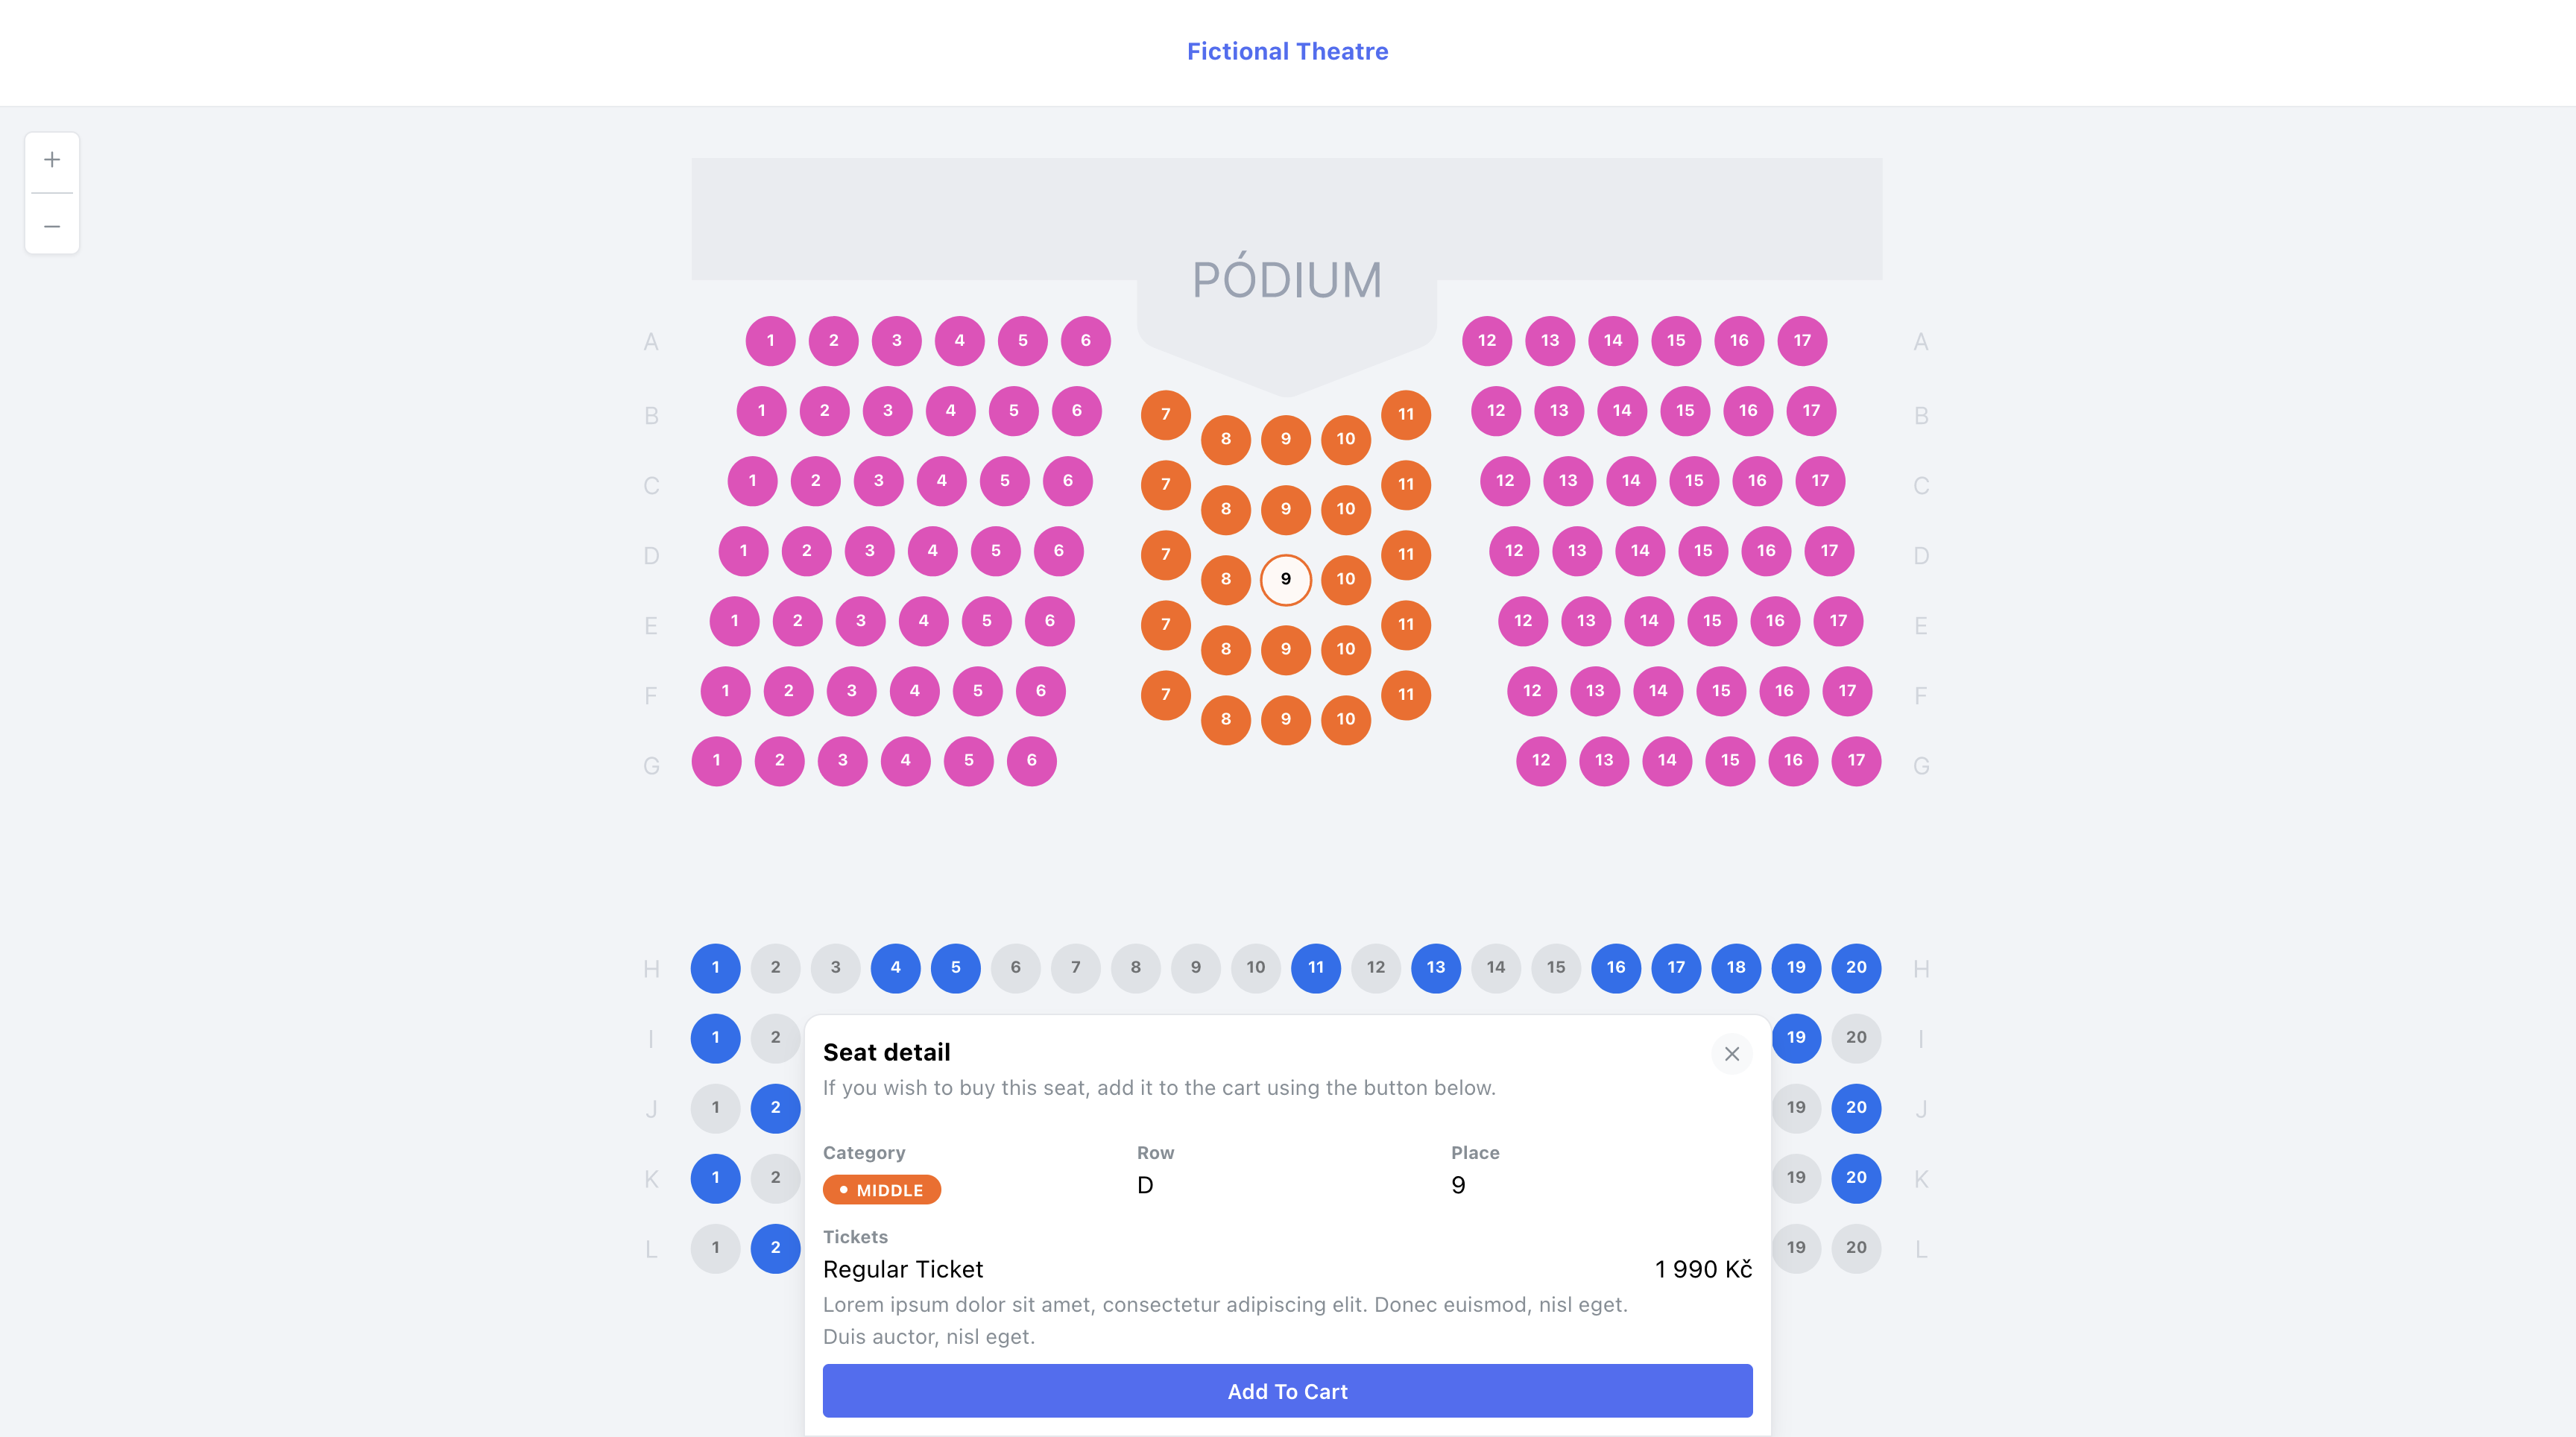
\includegraphics[width=\textwidth]{\FIGDIR/seating-map-seat}
	\caption{Snímek obrazovky interaktivní mapy sedadel}
	\label{fig:seating-map-seat}
\end{figure}

Obrázek~\ref{fig:seating-map-seat} zobrazuje výsledný produkt, ilustrující uživatelsky přívětivé rozhraní a dynamickou mapu sedadel.
Kombinace výše uvedených komponent umožňuje snadnou navigaci sedadel místa, okamžitý přístup k informacím o vstupenkách a přehlednou správu vstupenek, což vede k efektivnímu a příjemnému uživatelskému zážitku.
